\documentclass{standalone}
\usepackage{tikz}
\begin{document}

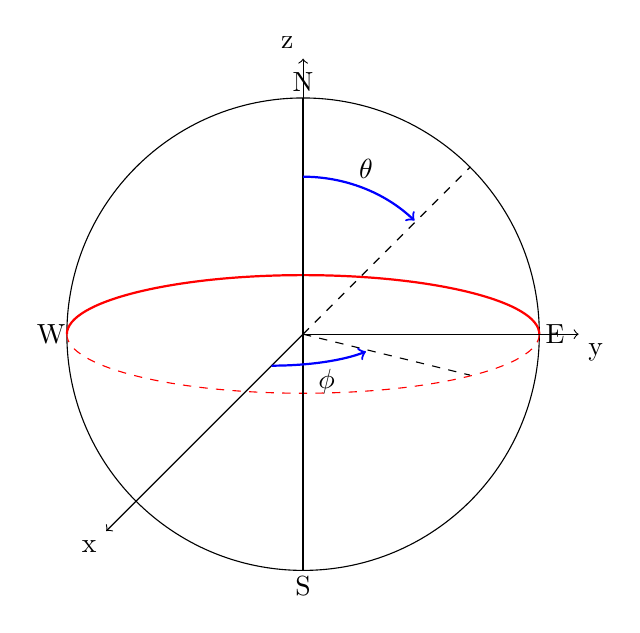
\begin{tikzpicture}
    % Draw the sphere
    \draw (0,0) circle (3);
    
    % Draw the equator
    \draw[red, thick] (3,0) arc (0:180:3 and 0.75);
    \draw[dashed, red] (-3,0) arc (180:360:3 and 0.75);
    
    % Draw the prime meridian
    \draw[thick] (0,-3) -- (0,3);
    
    % Draw latitude and longitude lines
    \draw[dashed] (0,0) -- (2.12,2.12);
    \draw[dashed] (0,0) -- (2.12,-0.52);
    
    % Labels for directions
    \node at (0,3.2) {N};
    \node at (0,-3.2) {S};
    \node at (3.2,0) {E};
    \node at (-3.2,0) {W};
    
    % Draw axes
    \draw[->] (0,0) -- (3.5,0) node[anchor=north west] {y};
    \draw[->] (0,0) -- (0,3.5) node[anchor=south east] {z};
    \draw[->] (0,0) -- (-2.5,-2.5) node[anchor=north east] {x};
    
    % Draw arc for latitude
    \draw[blue, thick, ->] (-0.4,-0.4) arc (-90:-37:1.5 and 0.45);
    \node at (0.3,-0.6) {$\phi$};
    
    % Draw arc for longitude
    \draw[blue, thick, ->] (0,2) arc (90:45:2 and 1.9);
    \node at (0.8,2.1) {$\theta$};

    
\end{tikzpicture}

\end{document}
